\textcolor{red}{Parlare dei big data, in particolare dei problemi con la quantità di dati e necessità di mettere ordine, dare significato\\
	prendere spunto da articolo and what can context do for data\\
	trovare grafici\\
	obiettivi della tesi}

Negli ultimi dieci anni si è assistito a un'enorme diffusione di Internet e soprattutto ad una varietà di dispositivi con i quali è possibile accederci. Agli albori esistevano solamente PC desktop con i quali poter visitare pagine per lo più statiche.

Ai giorni d'oggi invece sono disponibili dispositivi come smartphone e tablet che ci permettono di essere sempre connessi. L'incremento della velocità delle connessioni e il progresso tecnologico ha fatto sì che sia possibile consultare qualsiasi tipo di informazione su internet, che sia del semplice testo fino a immagini, video, ecc.

\begin{figure}[ht]
	\centering
	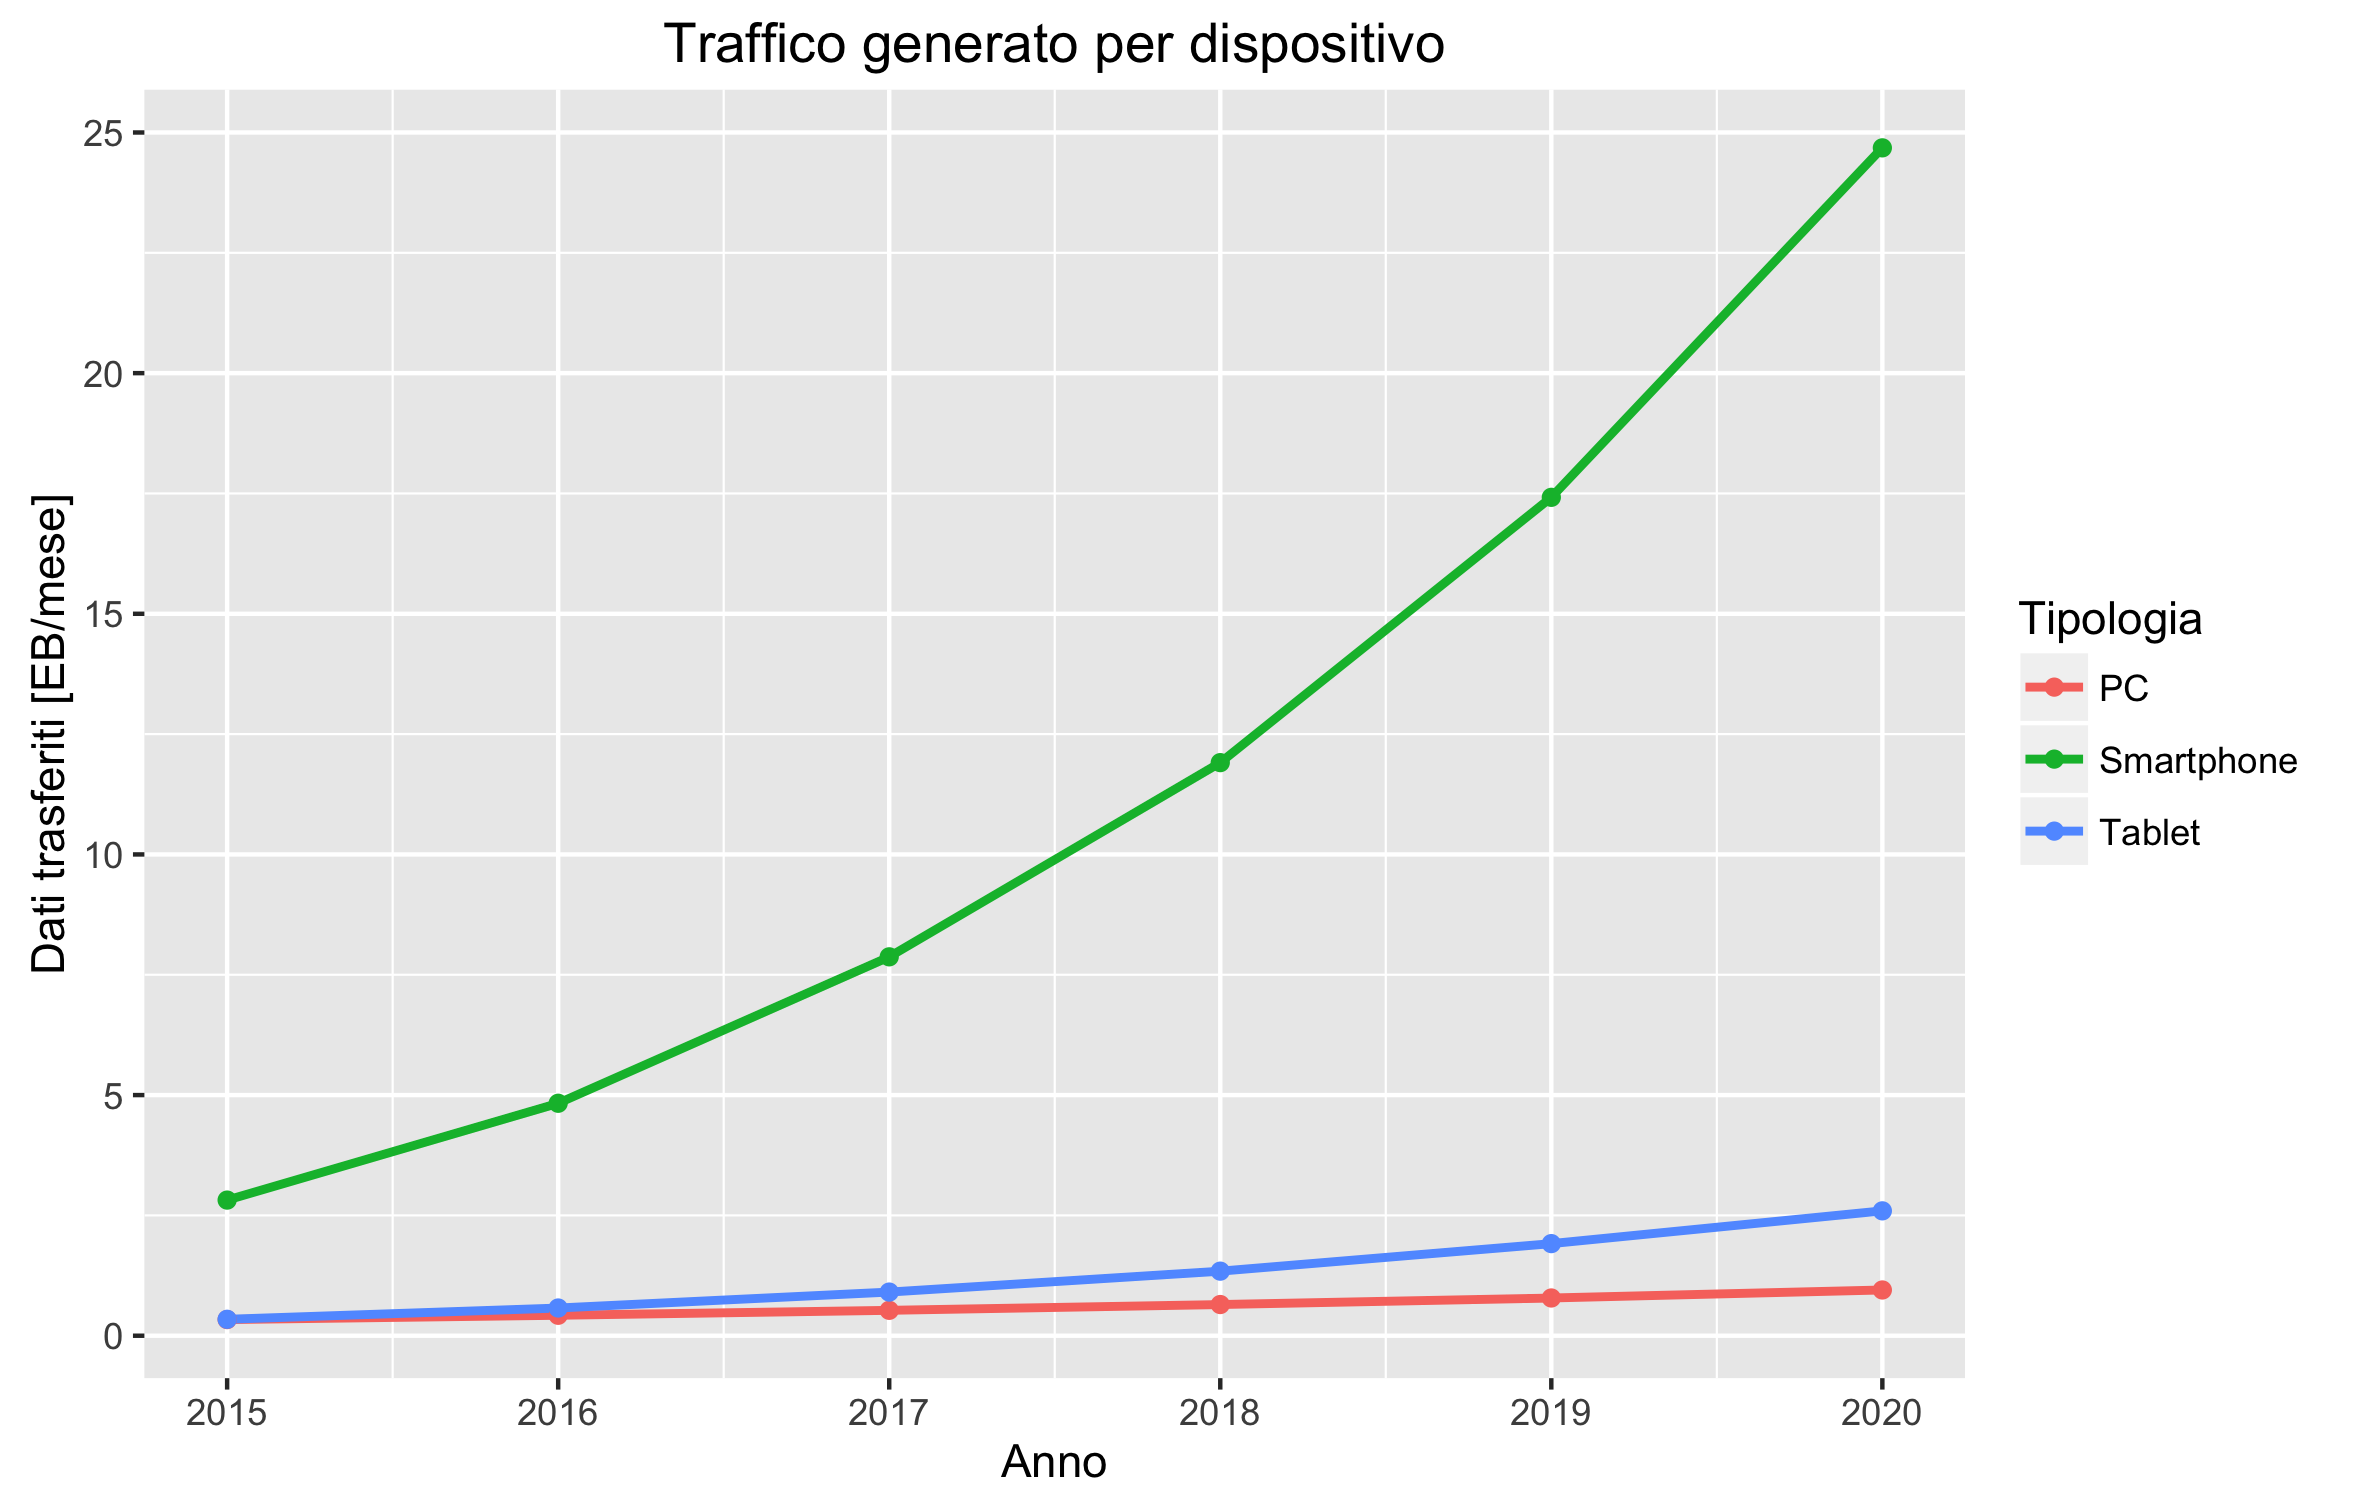
\includegraphics[width=\textwidth]{1-introduzione/immagini/traffico-dispositivi.png}
	\caption[Traffico generato per tipologia di dispositivo]{Traffico generato per tipologia di dispositivo (fonte: Cisco, 2016)\label{fig:traffico-tipologia-dispositivo}}
\end{figure}

Si è persa anche la tradizione che ci sia un gestore che pubblica contenuti in quanto ormai sono direttamente gli utenti a produrre la maggior parte delle informazioni disponibili. Questo fenomeno è stato accentuato con la creazione dei \emph{social network}, che permettono di creare collegamenti tra le persone dove è possibile condividere qualunque cosa che ognuno trova interessante.

\begin{figure}[ht]
	\centering
	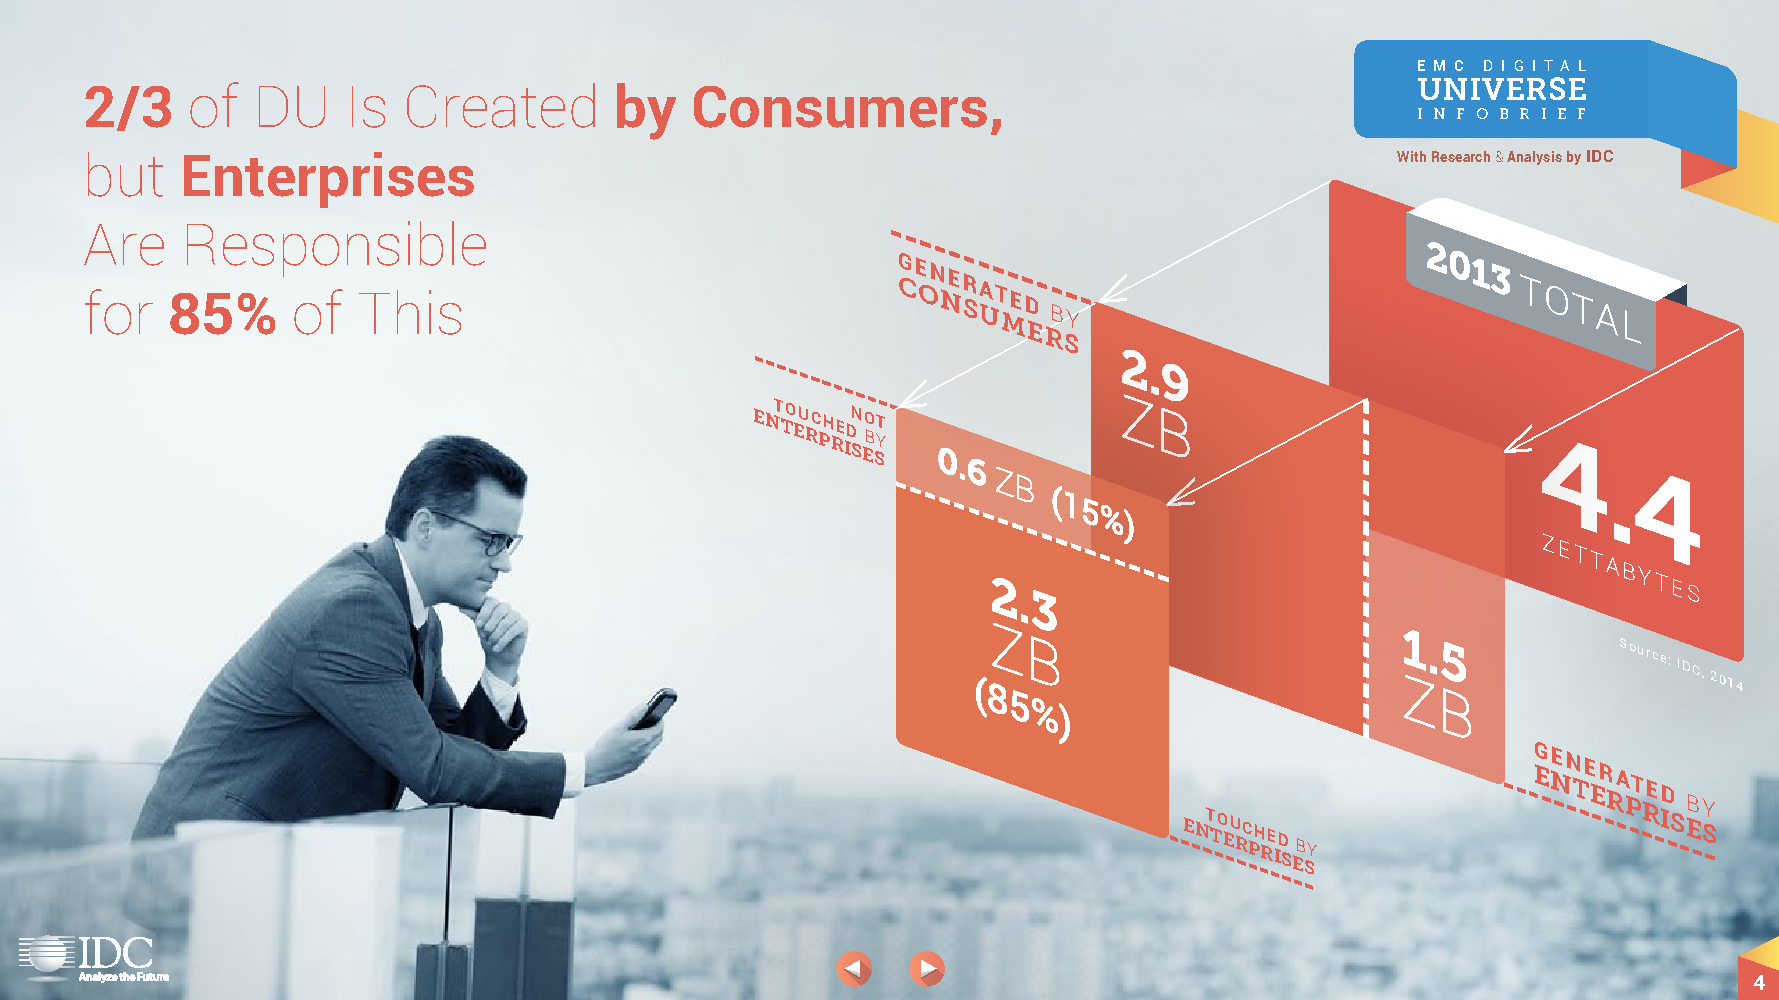
\includegraphics[width=\textwidth]{1-introduzione/immagini/dati-generati-consumer.pdf}
	\caption[Analisi della quantità di dati generati]{Analisi della quantità di dati generati (fonte: IDC, 2014)\label{fig:analisi-dati-generati}}
\end{figure}

\upe sempre maggiore anche il traffico legato ai video o alla musica, grazie a servizi che permettono lo \emph{streaming} dei contenuti come YouTube, Spotify, Netflix, ecc. \textcolor{red}{aggiungere siti web} 

\textcolor{red}{dati Cisco su traffico video}

Internet è diventato una fonte immensa di informazioni che è destinato sempre ad aumentare. Un recente trend è relativo ai dispositivi connessi, definito \emph{Internet of Things}. L'idea è che qualsiasi dispositivo può essere connesso a Internet per generare informazioni, in particolare tutti quelli provvisti di \emph{sensori} che possono fornire informazioni sullo stato dell'ambiente nel quale si trovano.

\begin{figure}[ht]
	\centering
	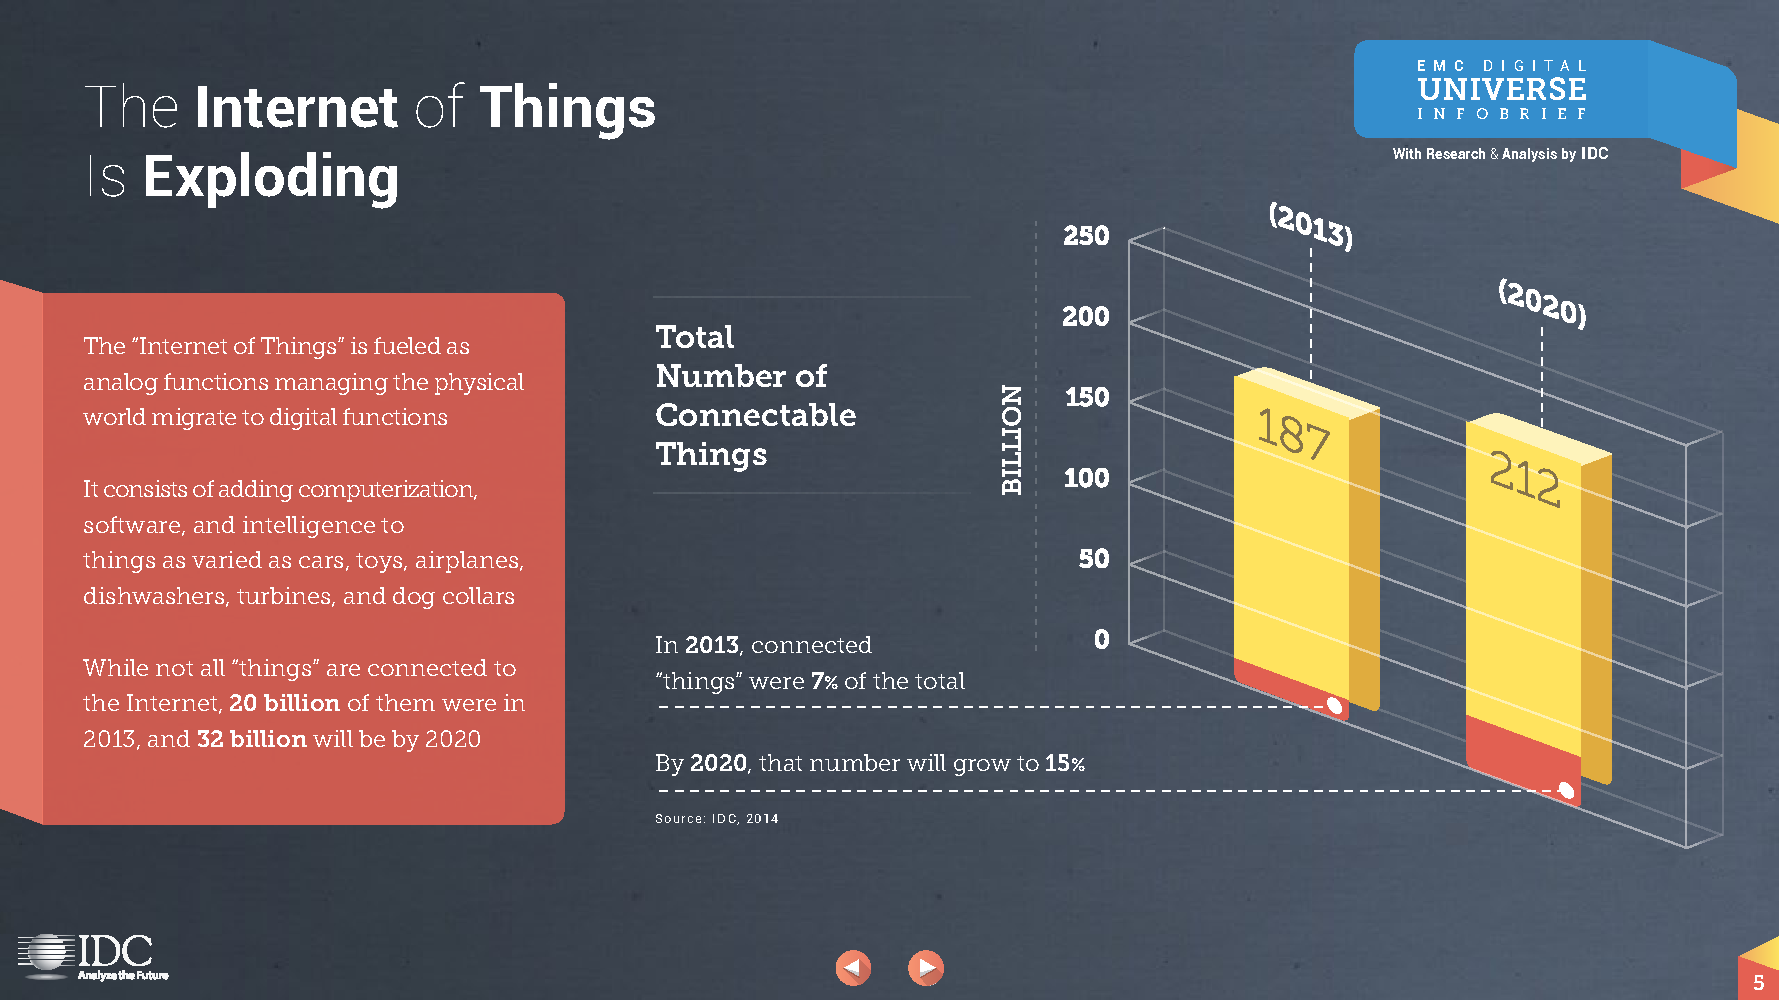
\includegraphics[width=\textwidth]{1-introduzione/immagini/iot-trend.pdf}
	\caption[Statistiche sull'Internet of Things]{Statistiche sull'Internet of Things (fonte: IDC, 2014)\label{fig:statistiche-iot}}
\end{figure}

Questa è la \emph{Information Age}, cioè il fenomeno dove la conoscenza è alla base della società e la tecnologia influenza il modo in cui operano le industrie e gli operatori dei servizi, permettendogli di agire in modo più efficiente e conveniente. Tutte queste informazioni permettono a chiunque di esplorarle secondo le proprie esigenze. 

\textcolor{red}{parlare dei pro nell'acquisire informazioni da diverse fonti}

Il problema che ora si pone è quello che i ricercatori chiamano \virgolette{dare senso ai dati}, i quali danno un valore aggiunto solo utilizzando algoritmi appropriati. Possedere una grande quantità di dati senza poterli sfruttare è inutile. \upe necessario trarre vantaggio dalla possibilità di analizzarli, estrarre informazioni utili per ricavarne conoscenza. 

%Inizio parte del contesto
Questo aumento della quantità di informazioni, se non propriamente controllato, può provocare un ammasso di dati che genera soltanto confusione piuttosto che fornire elementi utili, riducendo i benefici che invece si potrebbero ricavare da tutte queste informazioni. Tuttavia, distinguere le informazioni rilevanti da quelle che non lo sono è un compito tutt'altro semplice; alcune informazioni potrebbero essere trattate in maniera differente, anche per lo stesso utente, che in diverse situazioni o posti ha bisogno di informazioni differenti. 

\textcolor{red}{Descrivere un po' il contesto}

%Resta aperto il problema di come visualizzare le operazioni e come ricercare le info in modo semplice (Fornire interfaccia per permettere agli utenti di cercare le informazioni)

Il contesto permette dunque di acquisire informazioni rilevanti per l'utente, ma non definisce nessuna regola su come verranno visualizzati all'utente finale. Con la diffusione di dispositivi mobili sempre più sofisticati si è resa maggiormente necessaria un'esperienza utente semplice che lo guidi durante le sue attività 

\textcolor{red}{Ruolo dell'user experience}

Vengono dunque in soccorso i \emph{Mashup}, che permettono la realizzazione di interfacce grafiche estremamente dinamiche. In questo modo può essere facilmente rappresentato il contesto e definire un aspetto idoneo per le varie categorie di risultati. \textcolor{red}{Ogni categoria di informazioni ha le sue peculiarità e avere schemi diversi per categoria di dati ha il suo perché}



\section{Struttura della tesi\label{sec:struttura-tesi}}




\textcolor{red}{descrivere struttura della tesi}